\begin{titlingpage}
  \begin{center}
    \vspace*{1in}

    \textbf{\large MA112:\\Discrete Mathematics}

\vspace*{1in}

    Waleed A. Yousef, Ph.D.,

    \bigskip

    Human Computer Interaction Lab.,\\Computer Science Department,\\Faculty of Computers and Information,\\Helwan University,\\Egypt.

    \bigskip

    \today
  \end{center}
\end{titlingpage}

\textbf{Lectures follow:}

\bibentry{Rosen2007DiscMath}

\begin{center}
  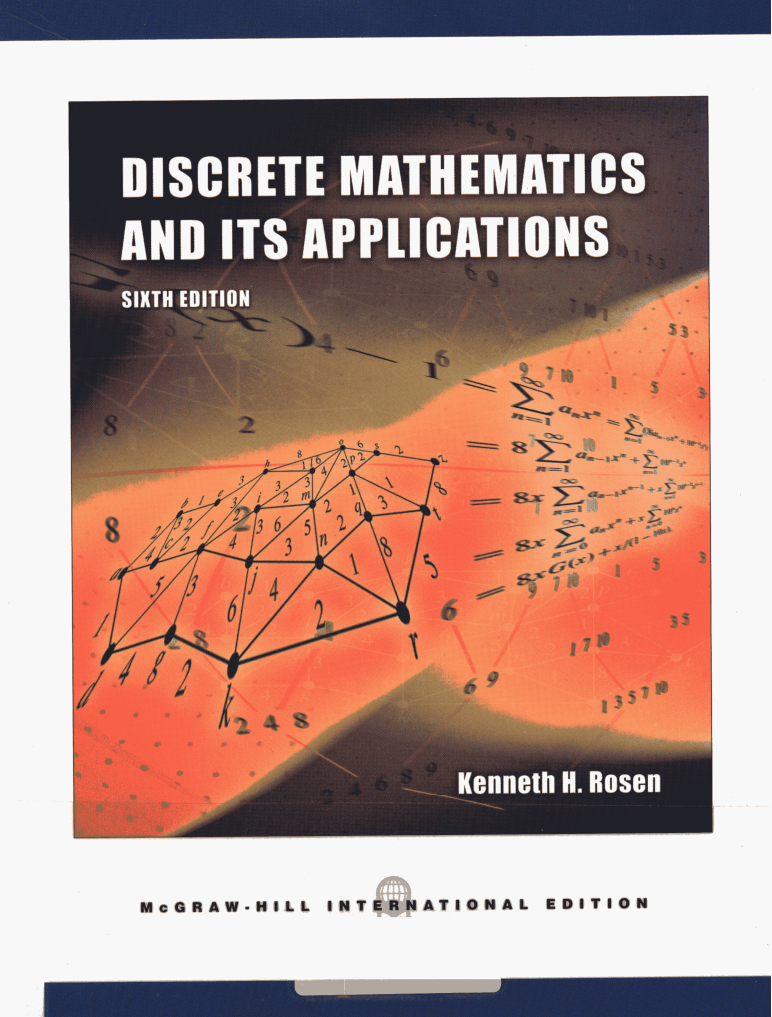
\includegraphics[width=.4\textwidth]{../Graphics/FrontMatter/BookFrontCover.png}
\end{center}

\chapter*{Course Objectives}

\begin{itemize}
  \item Developing rigorous treatment.
  \item Developing mathematical foundations to CS.
  \item Building intuition.
  \item Linking to CS applications (Rosen has great practical examples)
  \item Introducing students to ``Mathematical Computing'' (we will use ``Sage'')
\end{itemize}

\textbf{Let's see how Mathematics is the pillars of Engineering and CS by illustrating the book's chapters}

\clearpage
{
  \tiny
  \settocdepth{subsection}
  \tableofcontents
}


%%% Local Variables:
%%% mode: latex
%%% TeX-master: "../LectureNotesMA112"
%%% End:
